\chapter{Introduction}

\section{Background and Motivation}
A modern steel manufacturing facility has a complex organization consisting of various workstations and can handle different jobs simultaneously. Facility systems are based on Computer Integrated Manufacturing (CIM) implemented in workstations in an automated fashion with combined computer control and digital information~\cite{waldner1992}. The sensory information received from workstation equipment is stored as data within a server to be incorporated with planning progress to provide functionality, adaptability and effective resource allocation in manufacturing processes~\cite{Saadaoui2019}.

 \begin{figure}[!ht]
	\begin{center}
		\makebox[\textwidth]{
			\centering
			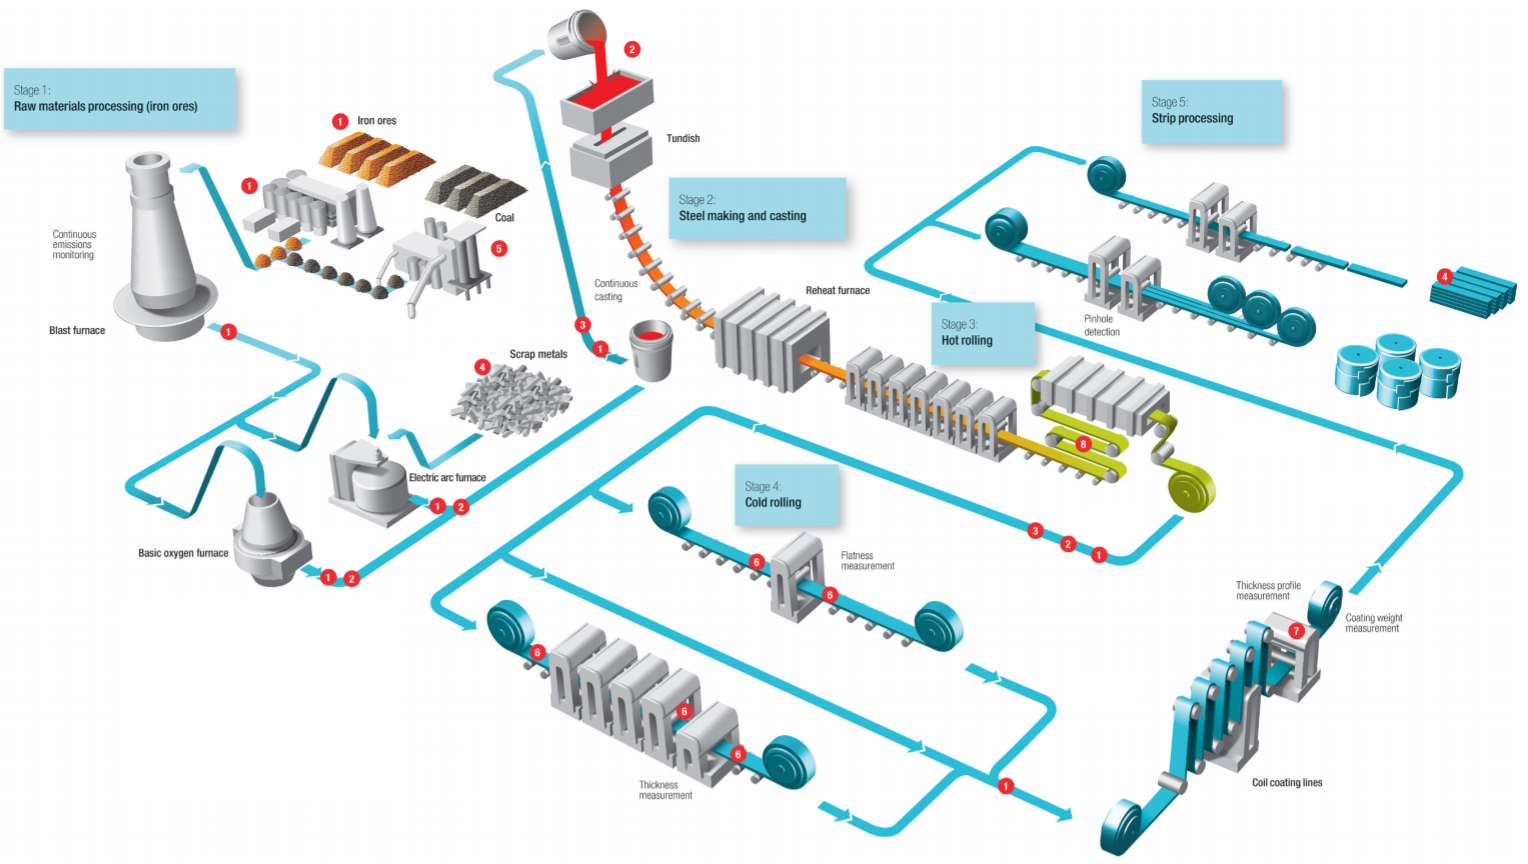
\includegraphics[width=1.0\linewidth]{../images/steel-production-steps.png}}
		\caption{Steel Manufacturing Steps~\cite{sinha-spinks_2015}.}
		\label{figure-steel-production-steps}
	\end{center}
\end{figure}

Fundamental steel manufacturing steps with respective production units are shown in Fig.~\ref{figure-steel-production-steps}. Raw materials are melted in the blast, electric arc or basic oxygen furnaces to obtain liquid iron. Accordingly, liquid steel alloy is sent to the continuous casting line, where it is poured into a mould cavity until it cools and solidifies. The solid material is sent to a further step, the rolling process, which can be performed in two different modes: hot rolling and cold rolling. It allows obtaining the material's desired mechanical properties, uniform thickness, a control on width dimension, and converting material to a flat and rectangular slab, a semi-finished steel product. The solid material is heated in a reheat furnace before it's pressed in the hot rolling unit. The cold rolling unit improves surface finish and flatness, and it allows to modify metal work hardening. The output slabs of the rolling process might be converted into compact coils featuring high lengths unless they won't be sent to further process units on the continuous production line. Pickling is a treatment to remove rust and impurities on the slab surface; it is applied before cold rolling processes and makes it easier to work on the material. Hot-dip galvanizing process is an effective coil coating technique. Galvanizing is an application of protective zinc coating on the steel surface to improve corrosion resistance.

The above-explained processes and workstations can be arranged in various compact plant solutions based on the requirements of different facility organizations or demands. Table~\ref{Tab: production_lines} shows four separate production lines that the SMS group supplied to the steel manufacturing facility: Big River Steel, located in Arkansas, USA~\cite{BRS}.
\begin{table}[ht!]
	\centering
	\setlength{\arrayrulewidth}{0.75pt}% 
	\begin{tabular}{|c|c|c|}
		\hline
		\rowcolor[HTML]{FFFFC7} 
		\makecell{Label in\\Fig.~\ref{figure-steel-production-steps}} & Production Unit / Plant                       & Description                                                                                    \\ \hline
		A               & \makecell{Continuous Casting\\Machine (CCM)}            & \makecell{Mould steel cools and \\  solidifies, passing through \\the mould cavity.}                          \\ \hline
		B               & \makecell{Compact Strip \\Production (CSP)}              &\makecell{Compact plant including CCM,\\   reheating furnace, hot rolling unit \\and strip processing unit.}       \\ \hline
		C               & \makecell{Pickling Line \& Tandem \\Cold Mill (PLTCM)} & \makecell{Compact plant including a\\   turbulence pickling section \\and a tandem mill.}                     \\ \hline
		D               & \makecell{Continuous Galvanizing \\Line   (CGL)}         & \makecell{Application of protective zinc \\  coating on the steel surface to \\improve corrosion resistance.} \\ \hline
	\end{tabular}
	\caption{Production Lines Including Various Machine Modules and Compact Solutions}
	\label{Tab: production_lines}
\end{table}

{\color{red}
	
	Each process has its own technical or physical constraints considering the above-explained production steps. Constraints arise from those technology-driven production types related to facility capabilities~\cite{cowling2001design}.
	
	Optimizing individual sequences in each process is a necessity for a successful local unit. Local constraints on different production units are integral parts of a global optimization problem that human expert planners tackle for a solution. The sequences produced in production lines are available as data output, so-called 'imprints' of what has been on sequence designers' minds. Therefore, looking at the historical production data and investigating the properties of those order sequences that have already been produced give indirect access to the patterns related to human experts' knowledge systems. The technical and physical constraints mentioned in the introduction section are unique to those specific production lines, and they vary under differently customized production lines. Produced order properties such as thickness, width, temperature, and chemical composition are the characteristic features of order products that are possibly shaped under the effect of those constraints. An investigation on the features of orders in the identical production sequences and comparing them might give interesting clues about related constraints and correspondingly provide patterns about human experts' decision strategies.
	
	I should discuss and refer to different constraints from the literature introduced for the manufacturing life cycle.
	
	As a motivation, I need to introduce different categories of constraints as technical constraints, performance-indicator based constraints to be quantified in the context of the FBA in the further steps of this work.
	
	Are logistic constraints, physical and chemical constraints coupled to topological features of the association network?
}

\section{Research Objective}

{\color{red} 
	Our hypothesis: different types of constraints create non-random features in the association networks for different binning schemes. Networks derived from various types of binning. Do they show non-random features when I have performance constraints or other types of constraints?
	
	Two fundamentally different constraints acting on the manufacturing process: technology-driven constraints and load-driven constraints, were shaped hypothetically and defined as two distinguished network approaches: fixed step-sized and fixed bucket-sized networks.
	
	FSS graphs had high modularity. That means that the actual quantity I discretize creates the constraints, while in the case of FBS, it would be the volume of orders that makes my constraints. That summaries our hypothesis.
	
	Explanation of my hypothesis is a theoretical/conceptual framework as a starting point for the investigation. It is a well-defined valid object and based on facts. Moreover, it is structured to discriminate the two types of constraints in the statistical properties of the production data.
	
	The initial step of this master thesis work was to quantify the characteristics of two hypothetical types of constraints in industrial production: technology-driven constraints and load-driven constraints.
		
}

\section{Research Plan and Thesis Organization}

{\color{red} 
	Having a small simulation framework would help understanding mechanistically the difference between the two types of constraints. But data analysis would provide us some intuition on what to look at. How can even detect that some real data are impacted/shaped by these two types of constraints?
	
	If I could now, in some way, do this analysis in time windows across 2-3 years of production data, then I undoubtedly will encounter time windows where the load in the system was really high so I would expect that the other type of constraints also place a role.
	
	It is plausible either the tech constraints do not go away, the other type of constraints is present with varying strength/importance in the system.
	
	Optimization principles coming from Operations Research:
	
	Considering the system as a linear set of fluxes of material flows. Finding the pattern of material flow that maximizes the output. The advantage of this approach: the notion of constraints is already present in that framework.
	
	Can these constraints be properly discriminated?
	Is there a formal way of defining them and are there functional consequences?
	Do they impact how the system behaves?
	Can I distinguish the signature of these constraints in data?
	
	Modeling alternatives: OR Methods, Discrete Event Simulations
	
	
	
	Methods are introduced here as indicative of two fundamentally different constraints acting on the manufacturing process: technological constraints on the one hand and constraints related to material flow and production capacity on the other.
	
	I plan to quantify the characteristics of two hypothetical types of constraints with an Operations Research Model consisting of two steps. First, analyzing the statistical properties of association networks over Time in an extensive data set from steel manufacturing; second, developing an abstract theoretical framework to understand better the connection between each type of constraint and the statistical patterns created by them. 
	
	Formulate the binning methods here because this will describe the hypothesis underlining my thesis.
	
	My Operations Research Model (OR model) combines Steel Manufacturing Events Analysis and Flux Balance Analysis. The art form of this model is to structure a standard data format and a shared analysis logic that allows comparing the results from manufacturing data and simulation data.
}